\documentclass[border=10pt]{standalone}
\usepackage{pgf,tikz,pgfplots}
\usetikzlibrary{quotes, angles}
%\usepackage{unicode-math}
%\setmainfont[Ligatures={TeX,Common}]{TeX Gyre Pagella}
%\setmathfont{TeX Gyre Pagella Math}
\usetikzlibrary{positioning}
\usetikzlibrary{arrows.meta}
\usetikzlibrary{calc, shapes, automata}
\tikzset{%
	% Specifications for style of nodes:
	base/.style = {rectangle, rounded corners, draw=black,
		%		minimum width=4cm, minimum height=1cm,
		inner sep=15pt,
		text centered, font=\sffamily}, 
	activityStarts/.style = {base, fill=blue!30},
	startstop/.style = {base, fill=red!30},
	activityRuns/.style = {base, fill=red!30},
	process/.style = {base, minimum width=2.5cm, fill=orange!15,
		font=\ttfamily},
}
\begin{document}
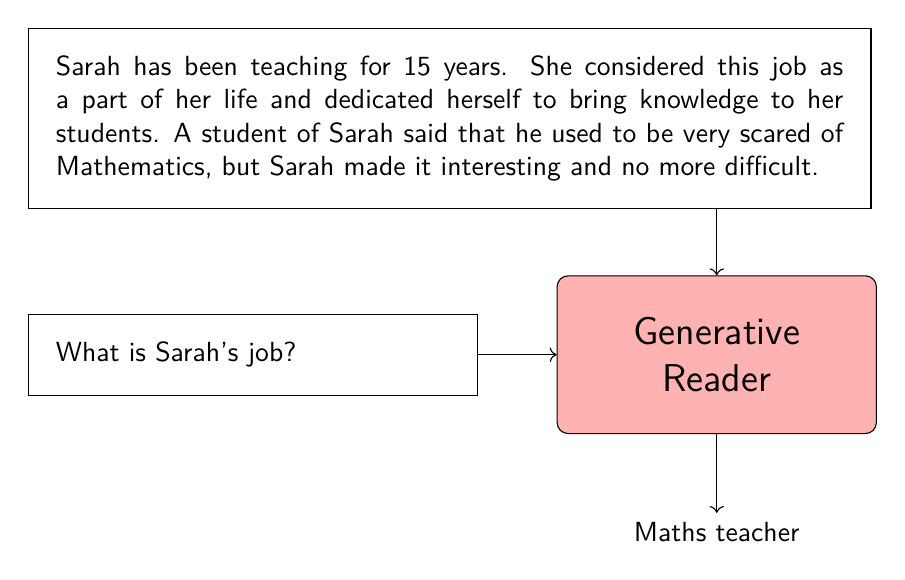
\begin{tikzpicture}[node distance=1.5cm,
	every node/.style={fill=white, font=\sffamily}, align=center]
	
	\node (ctxs) [right, text width=10cm, align=justify, draw=black, inner sep=10pt] {Sarah has been teaching for 15 years. She considered this job as a part of her life and dedicated herself to bring knowledge to her students. A student of Sarah said that he used to be very scared of Mathematics, but Sarah made it interesting and no more difficult. 
	};
	\node (query) [right, draw=black, inner sep=10pt, align=justify, text width=5cm, below=3cm of ctxs.west, anchor=west] {What is Sarah's job?};
	\node (reader) [activityRuns, right=1.cm of query, text width=3.cm] {\fontsize{14pt}{\baselineskip}\selectfont Generative\\[5pt] Reader};
	\draw[->] (query) -- (reader);
	\path let
	\p1 = (ctxs.south),
	\p2 = (reader.north)
	in
	coordinate (ctxsAnchor) at (\x2, \y1);
	\draw [->] (ctxsAnchor) -- (reader.north);
	\node (output) [below=1cm of reader] {Maths teacher};
	\draw [->] (reader.south) -- (output);
\end{tikzpicture}
\end{document}